\documentclass[14pt]{report}

% Настройки для поддержки русского языка
\usepackage[T2A]{fontenc}
\usepackage[utf8]{inputenc}
\usepackage[russian]{babel}

\usepackage{amsmath}
\usepackage{amssymb}
\usepackage{hyperref}
\usepackage{graphicx}
\usepackage{pgfplots}
\usepackage{pgfplotstable}
\usepgfplotslibrary{groupplots}
\usetikzlibrary{calc}
\pgfplotsset{width=15cm,compat=1.18}
\usepackage{booktabs}
\usepackage{autobreak}
\usepackage{breqn}

% Поля
\usepackage[lmargin=30mm, rmargin=15mm, tmargin=20mm, bmargin=20mm]{geometry}

% Межстрочный интервал 1.5
\usepackage{setspace}
\onehalfspacing

% Абзацный отступ 1.25 см
\usepackage{indentfirst}
\setlength{\parindent}{1.25cm}

% Шрифт Times New Roman (имитация для pdflatex)
\usepackage{mathptmx}

% Выравнивание по ширине
\usepackage{ragged2e}
\AtBeginDocument{\justifying}

% Заголовки по центру, строчные (кроме первой прописной) – для report:
\usepackage{titlesec}
\titleformat{\chapter}{\normalfont\bfseries}{\thechapter.}{1em}{\Large}
\titleformat{\section}{\centering\normalfont}{\thesection.}{1em}{\Large}
\titleformat{\subsection}{\centering\normalfont}{\thesubsection}{1em}{\large}
% \titleformat{\subsubsection}{\centering\normalfont\normalsize}{}{0pt}{}


% See https://www.overleaf.com/learn/latex/Pgfplots_package#Reducing_compilation_time
\usepgfplotslibrary{external}
\tikzexternalize

\graphicspath{{./src/}}

% Temporary workaround
% See https://github.com/matplotlib/matplotlib/issues/27907
\def\mathdefault#1{#1}
\everymath=\expandafter{\the\everymath\displaystyle}
\IfFileExists{scrextend.sty}{
  \usepackage[fontsize=10.000000pt]{scrextend}
}{
  \renewcommand{\normalsize}{\fontsize{10.000000}{12.000000}\selectfont}
  \normalsize
}

\begin{document}

\begin{abstract}
В работе рассматривается модификация классической схемы Лакса--Фридрихса для численного решения уравнения переноса. Предложено семейство разностных схем, параметризованное величиной $\sigma$, позволяющее варьировать диссипативные свойства метода. С использованием разложения по Тейлору и коррекции старших членов ошибки на пятиточечном шаблоне построена схема повышенного порядка аппроксимации.

Проведен детальный анализ устойчивости схемы методом фон~\mbox{Неймана}. С применением систем компьютерной алгебры (СКА) на базе библиотеки \texttt{sympy} (Python) получено аналитическое представление множителя перехода и исследована зависимость области устойчивости от параметров схемы $(\nu, \sigma)$. Установлены необходимые и достаточные условия устойчивости.

Численно исследован порядок сходимости схемы, подтверждающий теоретические оценки. Схема сравнивается со сквозными разностными схемами, в частности, со схемой Русанова третьего порядка. Для подавления нефизических осцилляций вблизи разрывов предложены два подхода к монотонизации: метод адаптивной искусственной вязкости и гибридная схема, комбинирующая решения высокого и низкого порядков.

Численные эксперименты демонстрируют эффективность предложенных методов как на гладких, так и на разрывных решениях.
\end{abstract}

\tableofcontents


\chapter{Введение}

Численное решение уравнений гиперболического типа, в частности, уравнения переноса, является фундаментальной задачей вычислительной математики с многочисленными приложениями в механике жидкости и газа, теории переноса излучения, моделировании процессов распространения примесей и других областях.

Классические разностные схемы для уравнения переноса обладают рядом известных недостатков. Схемы первого порядка (против потока, Лакса-Фридрихса) характеризуются высокой численной диффузией, приводящей к размытию фронтов и потере точности. Схемы второго порядка (Лакса-Вендроффа) обладают меньшей диффузией, но генерируют нефизические осцилляции вблизи разрывов решения, что может приводить к нарушению монотонности и появлению отрицательных значений в физически положительных величинах.

В связи с этим представляет интерес разработка численного метода, дающего монотонные решения с практически приемлемой точностью. Целью настоящей работы является построение и всестороннее исследование семейства явных разностных схем повышенного (третьего) порядка точности для линейного уравнения переноса, сохраняющих монотонность на разрывных решениях. Для достижения этой цели решаются следующие задачи: параметрическое обобщение схемы Лакса--Фридрихса с помощью параметра $\sigma$, теоретический анализ порядка аппроксимации с последующей коррекцией старших членов ошибки, строгое исследование устойчивости методом схемы, а также разработка алгоритмов подавления нефизичных осцилляций.

Научная новизна результатов заключается в постоении и исследовании однопараметрического семейства схем на основе схемы Лакса--Фридрихса, позволяющее плавно регулировать диссипативные и дисперсионные свойства. За счет привлечения пятиточечного пространственного шаблона и компенсации главных членов ошибки по Тейлору получена схема с локальным четвертым и интегральным третьим порядком аппроксимации. На основе символьных вычислений в СКА \texttt{sympy} выполнен исчерпывающий анализ устойчивости в двумерной области параметров $(\nu,\sigma)$, и аналитически определена граница максимально допустимого числа Куранта. Разработаны и сопоставлены два способа монотонизации схемы — метод адаптивной искусственной вязкости и гибридная схема с переключением порядка, что обеспечивает подавление осцилляций Гиббса при сохранении высокой точности в гладких областях.

Структура работы следующая. В разделе~\ref{sec:problem} формулируется постановка задачи. Раздел~\ref{sec:scheme} посвящен построению модифицированной разностной схемы и определению корректирующих коэффициентов. В разделе~\ref{sec:stability-analysis} проводится детальный анализ устойчивости методом фон~\mbox{Неймана}. Раздел~\ref{sec:convergence-analysis} содержит исследование порядка аппроксимации. В разделе~\ref{sec:monotonization} описываются методы монотонизации схемы для подавления осцилляций. Заключение~\ref{sec:conclusion} суммирует полученные результаты.

\chapter{Постановка задачи}
\label{sec:problem}

Рассматривается уравнение переноса в общем виде на прямоугольной области:
\begin{equation}
\frac{\partial u}{\partial t} + \operatorname{div}(\vec{a}\,u) = 0,
\label{eq:transport_general}
\end{equation}
где $u = u(x,y,t)$ --- искомая функция, $\vec{a}$ --- вектор скорости переноса.

В одномерном случае при постоянной скорости $a = \mathrm{const} > 0$ уравнение~\eqref{eq:transport_general} принимает вид:
\begin{equation}
\frac{\partial u}{\partial t} + a\,\frac{\partial u}{\partial x} = 0.
\label{eq:transport_1d}
\end{equation}

Уравнение~\eqref{eq:transport_1d} рассматривается при следующих условиях:
\begin{itemize}
\item область: $x \in [0, L]$, $t \in [0, T]$;
\item начальное условие: $u(x, 0) = u_0(x)$.
\end{itemize}

Уравнение~\eqref{eq:transport_1d} описывает перенос величины $u$ со скоростью $a$ вдоль оси $x$ без изменения формы профиля. Точное решение имеет вид:
\begin{equation*}
u(x,t) = u_0(x - at).
\end{equation*}

% ===================
\chapter{Построение разностной схемы}
\label{sec:scheme}

Введём на рассматриваемой области $[0,L]\times[0,T]$ равномерную пространственно-временн\'{у}ю сетку
\begin{equation*}
x_i = i\Delta x,\quad i=0,\dots,N_x,\qquad 
t^n = n\Delta t,\quad n=0,\dots,N_t,
\end{equation*}
где $\Delta x = L/N_x$, $\Delta t = T/N_t$, и будем обозначать $u_i^n \approx u(x_i,t^n)$.

\section{Базовый метод Лакса--Фридрихса}
Классическая схема Лакса--Фридрихса имеет вид:
\begin{equation}
u_i^{n+1} = \frac{1}{2}(u_{i+1}^n + u_{i-1}^n) 
            - \frac{a\Delta t}{2\Delta x}(u_{i+1}^n - u_{i-1}^n),
\label{eq:lax-friedrichs}
\end{equation}
и может быть записана в консервативной форме
\begin{equation*}
u_i^{n+1} = \frac{1}{2}(u_{i+1}^n + u_{i-1}^n) 
            - \frac{a\Delta t}{\Delta x}\bigl(W^n_{i+1/2} - W^n_{i-1/2}\bigr),
\end{equation*}
где $W^n_{i\pm1/2}$~--- численные потоки, определённые соответствующим образом.

\section{Модификация с параметром}
Введём параметр $\sigma$ и модифицируем схему~\eqref{eq:lax-friedrichs}:
\begin{equation*}
u_i^{n+1} = \biggl[\,\sigma u_i^n 
            + (1-\sigma)\frac{u_{i+1}^n + u_{i-1}^n}{2}\biggr]
            - \frac{a\Delta t}{\Delta x}\bigl(W^n_{i+1/2} - W^n_{i-1/2}\bigr).
\end{equation*}

После раскрытия потоков разностное уравнение принимает форму:

\begin{equation}
u_i^{n+1} = \biggl[\,\sigma u_i^n 
            + (1-\sigma)\frac{u_{i+1}^n + u_{i-1}^n}{2}\biggr]
            - a\Delta t\,\frac{u_{i+1}^n - u_{i-1}^n}{2\Delta x}
            + \frac{a^2\Delta t^2}{2}\,
              \frac{u_{i+1}^n - 2u_i^n + u_{i-1}^n}{\Delta x^2}.
\label{eq:modified-expanded}
\end{equation}

\textbf{Замечание.} При $\sigma=1$ схема~\eqref{eq:modified-expanded} переходит в схему Лакса--Вендроффа второго порядка.

\section{Анализ ошибки аппроксимации}
Разложим значения в узлах по формуле Тейлора относительно точки $(x_i,t^n)$. Если решение достаточно гладкое, получаем дифференциальное приближение схемы~\eqref{eq:modified-expanded} (опустив индексы для простоты):

\begin{dmath}
u^{n + 1} = u - a \Delta t u_{x} + \left(\frac{\Delta x^{2}}{2} + \frac{a^{2} \Delta t^{2}}{2} - \frac{\sigma \Delta x^{2}}{2}\right) u_{xx} - \frac{a \Delta t \Delta x^{2} u_{xxx}}{6} + \left(\frac{\Delta x^{4}}{24} - \frac{\sigma \Delta x^{4}}{24} + \frac{a^{2} \Delta t^{2} \Delta x^{2}}{24}\right) u^{(IV)}_{xxxx} - \frac{a \Delta t \Delta x^{4} u^{(V)}_{xxxxx}}{120} + \left(\frac{\Delta x^{6}}{720} - \frac{\sigma \Delta x^{6}}{720} + \frac{a^{2} \Delta t^{2} \Delta x^{4}}{720}\right) u^{(VI)}_{xxxxxx} - \frac{a \Delta t \Delta x^{6} u^{(VII)}_{xxxxxxx}}{5040} + \frac{a^{2} \Delta t^{2} \Delta x^{6} u^{(VIII)}_{xxxxxxxx}}{40320} + \ldots,
\label{eq:TE}
\end{dmath}

откуда можно выделить члены ошибки

\begin{dmath}
u_i^{n + 1} - u(x_i, t^{n + 1}) = \input{src/scheme-taylor-error.tex} + \ldots.
\label{eq:TE}
\end{dmath}

\section{Повышение порядка схемы}
Чтобы повысить порядок аппроксимации, необходимо аннулировать старшие члены ошибки. Для этого аппроксимируем третью пространственную производную на расширенном пятиточечном шаблоне:
\begin{equation}
\left(\frac{\partial^3 u}{\partial x^3}\right)_i
\approx A\,u_{i-2} + B\,u_{i-1} + C\,u_i + D\,u_{i+1} + E\,u_{i+2},
\label{eq:stencil}
\end{equation}
где коэффициенты $A,B,C,D,E$ выбираются из условия компенсации мешающих членов. Используя разложения
\begin{equation*}
\begin{aligned}
u_{i\pm1} &= u_i \pm \Delta x\,u_x' + \frac{\Delta x^2}{2}u_{xx}'' \pm \frac{\Delta x^3}{6}u_{xxx}''' + \frac{\Delta x^4}{24}u_{xxxx} + \dots,\\
u_{i\pm2} &= u_i \pm 2\Delta x\,u_x' + \frac{(2\Delta x)^2}{2}u_{xx}'' \pm \frac{(2\Delta x)^3}{6}u_{xxx}''' + \frac{(2\Delta x)^4}{24}u_{xxxx} + \dots,
\end{aligned}
\end{equation*}
и подставляя~\eqref{eq:stencil} с учётом структуры ошибки в~\eqref{eq:TE}, мы приходим к системе линейных уравнений относительно коэффициентов $A,\dots,E$. Эквивалентная матричная запись системы после сокращения параметров (вида $\Delta x^k/k!$) имеет вид:
% TODO -- переписать систему как расширенную матрицу.
\begin{equation*}
\left[\begin{matrix}1 & 1 & 1 & 1 & 1\\-2 & -1 & 0 & 1 & 2\\4 & 1 & 0 & 1 & 4\\-8 & -1 & 0 & 1 & 8\\16 & 1 & 0 & 1 & 16\end{matrix}\right] x = \
       \left[\begin{matrix}0\\0\\1 - \sigma\\\frac{a^{3} \Delta t^{3}}{\Delta x^{3}} - \frac{a \Delta t}{\Delta x}\\- \frac{a^{4} \Delta t^{4}}{\Delta x^{4}} + \frac{a^{2} \Delta t^{2}}{\Delta x^{2}} - 2 \sigma + 2\end{matrix}\right]
\end{equation*}
Данная система имеет единственное решение, параметризованное величиной $\sigma$, так как матрица коэффициентов является матрицей Вандермонда с попарно различными узлами.

\section{Итоговая разностная схема}
Выражая коэффициенты $A,\dots,E$ и подставляя полученный член в разностное уравнение, получаем окончательный вид схемы
\begin{dmath}
u_i^{n+1} =
\frac{u^n_{i - 2} \left(-1 + \sigma + \nu^{4} - \nu^{2} - 2 \nu + 2 \nu^{3}\right)}{24} - \frac{u^n_{i - 1} \left(-1 + \sigma + \nu^{3} + \nu^{4} - 4 \nu - 4 \nu^{2}\right)}{6} + \frac{u^n_i \left(3 + \sigma + \nu^{4} - 5 \nu^{2}\right)}{4} - \frac{u^n_{i + 1} \left(-1 + \sigma + \nu^{4} - \nu^{3} - 4 \nu^{2} + 4 \nu\right)}{6} + \frac{u^n_{i + 2} \left(-1 + \sigma + \nu^{4} - \nu^{2} - 2 \nu^{3} + 2 \nu\right)}{24},
\label{eq:scheme-cfl-form-stencil-form}
\end{dmath}
где $\nu = a\Delta t/\Delta x$~--- число Куранта.  

Расписав дифференциальное приближение, можно проверить, что главный член ошибки аппроксимации этой схемы даётся выражением
\begin{equation}
\frac{\Delta x^{4} \left(\sigma - 1\right) \frac{d^{4}}{d x^{4}} u{\left(x \right)}}{24}
\label{eq:principal-error-term}
\end{equation}
Таким образом, достигается высокий (третий) порядок аппроксимации по пространству при выполнении условия устойчивости и подходящем выборе параметра $\sigma$.

% =================
\chapter{Исследование устойчивости}
\label{sec:stability-analysis}

Анализ устойчивости проводится методом фон~Неймана (в предположении периодическими граничными условиями). Гармоническое возмущение на $n$-м временн\'{о}м слое записывается как $u_j^n = \lambda^n e^{i j\theta}$, где $\theta = k\Delta x$~--- волновое число, а $\lambda$~--- множитель перехода. Множитель перехода $G_{\sigma}(\theta,\nu)$ определяется отношением амплитуд гармоники на соседних слоях:
\begin{equation*}
G_{\sigma}(\theta, \nu) = \frac{u_j^{n+1}}{u_j^n}\Big|_{\,u_j^n = e^{i j\theta}}.
\end{equation*}

Ввиду громоздкости преобразований и аналитических выражений использовались символьные вычисления с помощью СКА, а некоторые выкладки приведены в общем виде для подобных схем на симметричных шаблонах.

\section{Множитель перехода}
Подстановка гармоники в разностную схему~\eqref{eq:scheme-cfl-form-stencil-form} даёт выражение

% \begin{align}
% \begin{autobreak}
% \frac{e^{- 2 i \theta}}{24} \left(\nu^{4} + 2 \nu^{3} - \nu^{2} - 2 \nu + \sigma + 4 \left(- \nu^{4} - \nu^{3} + 4 \nu^{2} + 4 \nu - \sigma + 1\right) e^{i \theta} + \left(6 \nu^{4} - 30 \nu^{2} + 6 \sigma + 4 \left(- \nu^{4} + \nu^{3} + 4 \nu^{2} - 4 \nu - \sigma + 1\right) e^{i \theta} + \left(\nu^{4} - 2 \nu^{3} - \nu^{2} + 2 \nu + \sigma - 1\right) e^{2 i \theta} + 18\right) e^{2 i \theta} - 1\right)
% \end{autobreak}
% \label{eq:amplification-factor}
% \end{align}

\begin{dmath*}
G_{\sigma}(\theta,\nu) =
\frac{e^{- 2 i \theta}}{24} \left(\nu^{4} + 2 \nu^{3} - \nu^{2} - 2 \nu + \sigma + 4 \left(- \nu^{4} - \nu^{3} + 4 \nu^{2} + 4 \nu - \sigma + 1\right) e^{i \theta} + \left(6 \nu^{4} - 30 \nu^{2} + 6 \sigma + 4 \left(- \nu^{4} + \nu^{3} + 4 \nu^{2} - 4 \nu - \sigma + 1\right) e^{i \theta} + \left(\nu^{4} - 2 \nu^{3} - \nu^{2} + 2 \nu + \sigma - 1\right) e^{2 i \theta} + 18\right) e^{2 i \theta} - 1\right)
,
\end{dmath*}

где $\nu = a\Delta t/\Delta x$~--- число Куранта.

Квадрат модуля множителя перехода $|G|^2$ имеет вид:
\begin{dmath*}
% \vert G\vert ^2 = \\
\frac{1}{36} \left(\nu^{8} \cos^{4}{\left(\theta \right)} - 4 \nu^{8} \cos^{3}{\left(\theta \right)} + 6 \nu^{8} \cos^{2}{\left(\theta \right)} - 4 \nu^{8} \cos{\left(\theta \right)} + \nu^{8} - 6 \nu^{6} \cos^{4}{\left(\theta \right)} + 28 \nu^{6} \cos^{3}{\left(\theta \right)} - 48 \nu^{6} \cos^{2}{\left(\theta \right)} + 36 \nu^{6} \cos{\left(\theta \right)} - 10 \nu^{6} + 2 \nu^{4} \sigma \cos^{4}{\left(\theta \right)} - 8 \nu^{4} \sigma \cos^{3}{\left(\theta \right)} + 12 \nu^{4} \sigma \cos^{2}{\left(\theta \right)} - 8 \nu^{4} \sigma \cos{\left(\theta \right)} + 2 \nu^{4} \sigma + 7 \nu^{4} \cos^{4}{\left(\theta \right)} - 48 \nu^{4} \cos^{3}{\left(\theta \right)} + 102 \nu^{4} \cos^{2}{\left(\theta \right)} - 88 \nu^{4} \cos{\left(\theta \right)} + 27 \nu^{4} - 2 \nu^{2} \sigma \cos^{4}{\left(\theta \right)} + 20 \nu^{2} \sigma \cos^{3}{\left(\theta \right)} - 48 \nu^{2} \sigma \cos^{2}{\left(\theta \right)} + 44 \nu^{2} \sigma \cos{\left(\theta \right)} - 14 \nu^{2} \sigma - 2 \nu^{2} \cos^{4}{\left(\theta \right)} + 12 \nu^{2} \cos^{3}{\left(\theta \right)} - 24 \nu^{2} \cos^{2}{\left(\theta \right)} + 20 \nu^{2} \cos{\left(\theta \right)} - 6 \nu^{2} + \sigma^{2} \cos^{4}{\left(\theta \right)} - 4 \sigma^{2} \cos^{3}{\left(\theta \right)} + 6 \sigma^{2} \cos^{2}{\left(\theta \right)} - 4 \sigma^{2} \cos{\left(\theta \right)} + \sigma^{2} - 2 \sigma \cos^{4}{\left(\theta \right)} + 8 \sigma \cos^{3}{\left(\theta \right)} - 16 \sigma \cos{\left(\theta \right)} + 10 \sigma + \cos^{4}{\left(\theta \right)} - 4 \cos^{3}{\left(\theta \right)} - 6 \cos^{2}{\left(\theta \right)} + 20 \cos{\left(\theta \right)} + 25\right).
\end{dmath*}

\section{Условие устойчивости}
Схема устойчива по фон~Нейману тогда и только тогда, когда
\begin{equation}
|G_{\sigma}(\theta,\nu)|^2 \le 1 \quad \forall\,\theta\in[0,2\pi].
\label{eq:stability-condition}
\end{equation}
Это эквивалентно требованию
\[
\max_{\theta\in[0,2\pi]} |G_{\sigma}(\theta,\nu)|^2 \le 1.
\]
Таким образом, задача сводится к нахождению области в пространстве параметров $(\nu,\sigma)$, где выполняется~\eqref{eq:stability-condition}.

На рис.~\ref{fig:amplification-factor-parameter-profile} показана зависимость $|G|^2$ от волнового числа $\theta$ при различных значениях параметра $\sigma$, а на рис.~\ref{fig:extremal-paramter-amplification-factor-parameter-profile}~--- поведение значений $|G|^2$ при более <<экстремальных>> значениях $\sigma \approx 1$, $\sigma > 1$. Для практических целей мы ограничиваемся $\nu, \sigma \in [0, 1]$, но такие визуализации позволяют лучше понять поведение множителя перехода.

\begin{figure}[ht]
\centering
% \scalebox{.4}{\input{src/amplification-factor-parameter-profile.pgf}}
\caption{Профиль $|G_{\sigma}(\theta,\nu)|^2$ для набора параметров $\sigma$.}
\label{fig:amplification-factor-parameter-profile}
\end{figure}

\begin{figure}[ht]
\centering
% \scalebox{.4}{\input{src/amplification-factor-parameter-profile-extreme.pgf}}
\caption{Значения $|G|^2$ для больш\'{и}х $\sigma$.}
\label{fig:extremal-paramter-amplification-factor-parameter-profile}
\end{figure}

\section{Анализ границы устойчивости}

При проведении анализа по методу фон~\mbox{Неймана} подстановка сеточных гармоник в разностную схему даёт множители $e^{\pm ik\theta}$. Для схем на симметричных шаблонах после вычисления $|G|^2 = G \cdot \overline{G}$ коэффициенты при $e^{i(k - m)\theta}$ и $e^{i(m - k)\theta}$, где $k, m \in \{-2, \dots, 2\}$, совпадают, в результате чего появляются выражения, состоящие из косинусов кратных углов:

\[
\cos\theta, \quad \cos 2\theta, \quad \cos 3\theta, \quad \cos 4\theta,
\]

каждое из которых является полиномом от $x = \cos\theta$ соответствующей степени. Из представлений через полиномы Чебышёва также мгновенно получается алгоритм для необходимых преобразований в более удобную форму.

Заметим, что схема симметрична относительно направления переноса. Если заменить $a \to -a$ (то есть $\nu \to -\nu$), то схема остаётся <<той же самой>> с точностью до направления:

\[
G(\theta, -\nu) = \overline{G(\theta, \nu)}
\]

Множитель перехода при смене знака скорости становится комплексно-сопряжённым. Из этого следует, что

\[
|G(\theta, -\nu)| = |G(\theta, \nu)| \quad \Rightarrow \quad |G|^2 \text{ --- чётная функция по }\nu.
\]

Поэтому при раскрытии $|G|^2$ все нечётные степени $\nu$ взаимно уничтожаются.

Таким образом, выражение $|G|^2$ симметрично относительно $\theta = \pi$, содержит только чётные степени $\nu$ и может быть записано как полином от $x=\cos\theta$ и $\nu^2$:
% TODO: P - 1 -> P 
\begin{equation*}
P(x,\nu) = |G_{\sigma}(\theta,\nu)|^2,\quad x\in[-1,1].
\end{equation*}
Степени полинома по переменным:
\[
\deg_{\nu^2} P \le 4,\qquad \deg_{x} P \le 4.
\]

Условие устойчивости требует, чтобы $\max\limits_{x\in[-1,1]} P(x,\nu) \le 1$. Для этого достаточно исследовать <<первые>> точки $(x, \nu)$ нарушения границы устойчивости~--- те, в которых достигается равенство. Анализ включает три этапа:
\begin{enumerate}
\item Проверка граничных точек $x = \pm 1$ (соответственно $\theta \in \{0, \pi\}$): находятся действительные корни полиномов 
\[
P(-1,\nu)-1\quad \text{ и }\quad P(1,\nu)-1.
\]
Они в точности задают интервалы, на которых соответствующие многочлены отрицательны. После чего остаётся лишь отсеять отрицательные значения $\nu$.

% (x, nu) or (sigma, nu)?
\item Поиск внутренних экстремумов: критические точки $(x,\nu)$, в которых

\[ P=1\quad \text{ и }\quad \frac{\partial P}{\partial x} = 0 \]

определяются как корни дискриминанта $\operatorname{Disc}_x(P-1)$ после избавления от константных кратных корней (при наличии которых дискриминант обнуляется).

\item Пересечение всех полученных интервалов задаёт границу устойчивости $\nu_{\max}(\sigma)$. \textbf{Замечание.} На практике при <<разумных>> значениях параметра $\sigma$ среди всех корней просто выбирается минимальное положительное значение $\nu$, которое и задаёт $\nu_{\max}(\sigma)$.
\end{enumerate}

Описанные полиномы для левой ($\theta = 0$) и правой ($\theta = \pi$) граничных точек интервала имеют соответственно виды

\begin{equation*}
P(1,\nu)-1 =
\input{./src/left-boundary-stability-condition-polynomial.tex}
\end{equation*}

и

\begin{equation}
P(-1,\nu)-1 =
\frac{4 \left(\nu^{4} - 4 \nu^{2} + \sigma - 1\right) \left(\nu^{4} - 4 \nu^{2} + \sigma + 2\right)}{9}.
\label{eq:right-boundary-stability-condition-polynomial}
\end{equation}

% TODO: Почему?
В общем случае, для симметричных шаблонов $x = 1$ ($\theta = 0$) является корнем $P - 1$ (вероятно, кратным). Зачастую ожидаемо, что такие полиномы имеют простое представление в силу работы с рациолнальными коээфициентами. 

Дискриминант полинома $P(x,\nu)-1$ по переменной $x$ (с точностью до исключения кратных константных корней) записывается как
\begin{dmath}
\operatorname{Disc}_x(P) = \frac{\nu^{12}}{81} - \frac{10 \nu^{10}}{81} + \frac{\nu^{8} \left(\sigma + 10\right)}{27} - \frac{4 \nu^{6} \left(3 \sigma + 7\right)}{81} + \frac{\nu^{4} \left(3 \sigma^{2} - 9 \sigma + 22\right)}{81} + \frac{2 \nu^{2} \left(\sigma^{2} - 1\right)}{27} - \frac{\sigma^{3}}{27} + \frac{\sigma^{2}}{9} - \frac{\sigma}{9} + \frac{1}{27}
\label{eq:discriminant}
\end{dmath}


Используя свойство результанта

\[
\deg_y\mathrm{Res}(f,g,x) \leq \deg_y{f}\deg_y{g}
\]

для взаимнопростых $f$, $g$ можно оценить степени вхождения параметров в дискриминант:

\begin{align}
\deg_{\nu} \operatorname{Disc}_x(P) & \le 4^2 = 16,\\[1em]
\deg_{\sigma} \operatorname{Disc}_x(P) & \le (1 + 1)^2 = 4.
\end{align}

Поэтому возможно аналитическое выражение $\sigma(\nu)$ из условия $\operatorname{Disc}=0$. На рис.~\ref{fig:discriminant-surface} изображена поверхность дискриминанта.

\begin{figure}[hb]
\centering
\scalebox{.8}{\input{src/discriminant-surface.pgf}}
\caption{Поверхность дискриминанта $\operatorname{Disc}_x(P)$ как функции от $(\nu,\sigma)$.}
\label{fig:discriminant-surface}
\end{figure}

В общем случае для конкретного метода (то есть при отсутствии или фиксации параметра) проанализировать интервал можно

\vspace{1em}

\begin{enumerate}
\item Найдя представление действительных корней $\nu_0 \in \mathbb{R}$ полинома $\operatorname{Disc}_x(P)$ и подставить их в $P$.

\vspace{0.5em}

\item Проверить наличие корня $x \in (-1, 1)$ для $P(x,\nu_0)-1$ с помощью, например, последовательностей Штурма на концах интервала.
\end{enumerate}

\vspace{1em}

Необходимые для этого операции поддерживаются современными СКА.

\section{Итоговое ограничение на число Куранта}
% TODO -- correct this
Объединяя все положительные критические значения, находим наименьшее из них, определяющее границу устойчивости $\nu_{\max}(\sigma)$. Результирующая кривая изображена на рис.~\ref{fig:cfl-bound-vs-parameter}.

\begin{figure}[ht]
    \centering
    \input{src/cfl-bound-vs-parameter.tikz}
    \caption{Максимально допустимое число Куранта $\nu_{\max}$ как функция параметра $\sigma$.}
    \label{fig:cfl-bound-vs-parameter}
\end{figure}

Таким образом, схема~\eqref{eq:scheme-cfl-form-stencil-form} устойчива при выполнении условия $\nu \le \nu_{\max}(\sigma)$. При выборе $\sigma$, например, в диапазоне $[0.5,\,1.0]$, максимальное допустимое число Куранта оказывается близким к единице, что сохраняет высокую эффективность метода.

% =============

\section{Диссипация и дисперсия}

На рис.~\ref{fig:dissipation-dispersion-profile} представлены зависимости модуля коэффициента перехода $|G|$ (амплитудная диссипация) и относительной фазовой ошибки (дисперсия) от безразмерного волнового числа $\theta = k\Delta x$ на отрезке $[0, \pi]$.


\begin{figure}[ht]
    \centering
    \input{src/dissipation-dispersion-profile.tikz}
    \caption{Диссипативные и дисперсионные свойства схемы при $\sigma = 0.5$ для различных значений числа Куранта $\nu$. Слева: модуль коэффициента перехода $|G|$ (диссипация). Справа: относительная фазовая ошибка (дисперсия).}
    \label{fig:dissipation-dispersion-profile}
\end{figure}

Левый график иллюстрирует диссипативные свойства численного метода. В длинноволновом пределе ($\theta \to 0$) для всех рассмотренных чисел Куранта выполняется условие $|G| \to 1$, что подтверждает аппроксимацию и согласованность схемы. На коротких волнах ($\theta \to \pi$) проявляется схемная вязкость, величина которой существенно зависит от $\nu$. Наибольшим диссипативным эффектом обладает схема при "средних" значениях $\nu$: модуль $|G|$ падает практически до нуля на высоких частотах, что способствует эффективному подавлению нефизичных коротковолновых осцилляций. Особого внимания заслуживает случай большего $\nu = 0.9$: на коротких волнах кривая $|G|$ превышает единицу, что наглядно демонстрирует потерю устойчивости схемы при превышении критического числа Куранта $\nu_{\max}$ для данного $\sigma$, что также подтверждает теоретические результататы.

Правый график демонстрирует дисперсионные характеристики схемы. Поведение относительной фазовой ошибки меняет свой характер в зависимости от числа Куранта. При меньших значениях $\nu$ ошибка отрицательна, что означает отставание численных гармоник от точного решения. При этом для "средних" $\nu$ дисперсионная ошибка остается близкой к нулю в широком диапазоне средних волн и резко возрастает лишь в коротковолновой части спектра. При б\'{о}льших значениях ошибка становится положительной, указывая на то, что численные волны опережают точное решение. 

Таким образом, анализ показывает, что выбор числа Куранта определяет не только устойчивость, но и характер ошибок схемы. Например, при $\sigma = 0.5$ "средние" значения $\nu$ обеспечивает отличные дисперсионные свойства для длинных и средних волн в сочетании с сильным диссипативным подавлением коротковолнового шума.

\chapter{Исследование порядка аппроксимации схемы}
\label{sec:convergence-analysis}

Теоретический анализ ошибки аппроксимации, проведённый в разделе~\ref{sec:scheme}, означает, что на одном временн\'{о}м шаге локальная ошибка схемы имеет \textbf{четвёртый порядок} по пространственному шагу $\Delta x$ (при фиксированном сеточном числе Куранта $\nu$). Однако при численном интегрировании уравнения переноса до конечного момента времени $T$ накопление локальной ошибки приводит к понижению порядка на единицу. Таким образом, интегральная ошибка (т.е. ошибка в момент $T$) должна демонстрировать сходимость порядка $O(\Delta x^3)$.

Для проверки этих оценок была проведена серия расчётов на последовательности сгущающихся равномерных сеток. Ошибки были измерены как нормы 

$$||e||_{L_p} = (\Delta x\sum_{i = 1}^n {e_i^p})^{1/p}$$

абсолютной разности точного и численного решений. В качестве теста использовалась задача о переносе гладкого начального профиля $\exp(-(x-a)^{2}/b^{2})$ с периодическими граничными условиями. В дальнейшей работе для проверки свойств схем использовались профили, описанные в ~\cite{galanin1999} с периодическими граничными условиями.
% Число Куранта фиксировалось равным $\nu = 0.1$, чтобы исключить влияние аппроксимации по времени.
Результаты сравнивались с классической схемой Лакса–Вендроффа, имеющей второй порядок аппроксимации.

\begin{figure}[ht]
    \centering
    \input{src/convergence-le.tikz}
    \caption{Зависимость локальной ошибки от шага сетки $\Delta x$ в двойном логарифмическом масштабе. Наклон прямой для предлагаемой схемы близок к 4, что подтверждает четвёртый локальный порядок. Для схемы Лакса–Вендроффа наблюдается второй порядок (наклон 2).}
    \label{fig:convergence-le}
\end{figure}

\begin{table}[h]
    \centering
    \label{tab:convergence-le}
    
    \begin{tabular}{l l c c c c c c}
\toprule
Method & Norm & 51 & 101 & 201 & 401 & 801 & 1601 \\
\midrule
Lax-Wendroff & $L_1$ & -2.87 & -5.77 & -8.74 & -11.73 & -14.72 & -17.72 \\
 & $L_2$ & -4.79 & -7.72 & -10.70 & -13.69 & -16.69 & -19.69 \\
 & $L_\infty$ & -6.14 & -9.04 & -12.01 & -15.00 & -18.00 & -21.00 \\
\midrule
LF-type & $L_1$ & -4.38 & -8.29 & -12.25 & -16.24 & -20.19 & -23.92 \\
 & $L_2$ & -6.33 & -10.23 & -14.20 & -18.19 & -22.15 & -24.73 \\
 & $L_\infty$ & -7.66 & -11.38 & -15.31 & -19.29 & -22.94 & -23.01 \\
\bottomrule
\end{tabular}
    
    % TODO: translate
    \caption{Convergence of Lax-Wendroff and LF-type schemes, errors are $\log_2$-scaled.}
\end{table}

\begin{figure}[h]
    \centering

    \input{src/convergence-le-diminishing-parameter.tikz}

    % TODO: change descr
    \caption{Зависимость локальной ошибки от шага сетки $\Delta x$ в двойном логарифмическом масштабе при стремлении старшего члена ошибки к 0 ($\sigma \to 1$).}
    \label{fig:convergence-le-diminishing-parameter}
\end{figure}

\begin{figure}[h]
\centering
    \input{src/convergence-ge.tikz}
    \caption{Интегральная ошибка в нормах $L_2$ и $L_\infty$ в конечный момент времени. Наклоны прямых для предлагаемой схемы соответствуют третьему порядку сходимости, в то время как схема Лакса–Вендроффа даёт второй порядок.}
    \label{convergence-ge}
\end{figure}

\begin{table}[h]
    \centering
    \label{tab:convergence-ge}
    
    \begin{tabular}{l l c c c c c c}
\toprule
Method & Norm & 51 & 101 & 201 & 401 & 801 & 1601 \\
\midrule
Lax-Wendroff & $L_1$ & 0.50 & -1.39 & -3.38 & -5.39 & -7.39 & -9.40 \\
 & $L_2$ & -1.54 & -3.36 & -5.34 & -7.35 & -9.36 & -11.36 \\
 & $L_\infty$ & -2.93 & -4.65 & -6.65 & -8.66 & -10.67 & -12.67 \\
\midrule
LF-type & $L_1$ & -1.20 & -3.93 & -6.90 & -9.91 & -12.91 & -15.91 \\
 & $L_2$ & -3.13 & -5.88 & -8.85 & -11.86 & -14.86 & -17.87 \\
 & $L_\infty$ & -4.51 & -7.04 & -9.96 & -12.95 & -15.96 & -18.96 \\
\bottomrule
\end{tabular}
    
    % TODO
    \caption{Convergence of Lax-Wendroff and LF-type schemes, errors are $\log_2$-scaled.}
\end{table}

Рисунок~\ref{fig:convergence-le} подтверждает четвёртый локальный порядок: при уменьшении $\Delta x$ локальная ошибка убывает пропорционально $\Delta x^4$. Рисунок~\ref{convergence-ge} демонстрирует, что интегральная ошибка во всех нормах уменьшается как $O(\Delta x^3)$, что полностью согласуется с теоретическим ожиданием $O(\Delta x^4 / \Delta t) = O(\Delta x^3)$ при фиксированном $\nu$, то есть $\Delta t \sim \Delta x$. Таким образом, предложенная схема обладает на порядок более высокой скоростью сходимости по сравнению со стандартным методом Лакса–Вендроффа, достигая интегрального третьего порядка точности.

\chapter{Монотонизация схемы}
\textsc{\label{sec:monotonization}
}
Схемы высокого порядка, подобные построенной в разделе~\ref{sec:scheme} не могут являться монотонными по теореме Годунова ~\cite{godunov1954} и склонны порождать нефизичные осцилляции (явление Гиббса) в окрестности резких градиентов и разрывов решения. На рисунке~\ref{fig:scheme-comparison-discontinuous} можно увидеть сравнение со схемой Русанова~\cite{rusanov1970}

\begin{dmath}
u_i^{n + 1} =
- \frac{u^n_{i - 2} \left(\omega - 2 \nu + 2 \nu^{3}\right)}{24} + \frac{u^n_{i - 1} \left(\omega + \nu^{3} - 4 \nu + 3 \nu^{2}\right)}{6} - \frac{u^n_i \left(-4 + \omega + 4 \nu^{2}\right)}{4} + \frac{u^n_{i + 1} \left(\omega - \nu^{3} + 3 \nu^{2} + 4 \nu\right)}{6} - \frac{u^n_{i + 2} \left(\omega - 2 \nu^{3} + 2 \nu\right)}{24}
\end{dmath}

Для подавления подобных осцилляций и придания схеме свойства монотонности применены два подхода: введение адаптивной искусственной вязкости и построение гибридной схемы.

\begin{figure}[ht]
\centering
\input{src/scheme-comparison-discontinuous.tikz}
\caption{Сравнение решений разными методами на разрывном шаблоне.}
\label{fig:scheme-comparison-discontinuous}
\end{figure}


\section{Адаптивная искусственная вязкость}

Идея, впервые предложенная Дж. фон Нейманом и Р. Рихтмайером в \cite{vonneumann1950}, состоит во введении в уравнение локального диссипативного слагаемого. Модифицированное уравнение имеет вид
\begin{equation}
\frac{\partial u}{\partial t} + a \frac{\partial u}{\partial x} 
= \frac{\partial}{\partial x}\left(\mu(x,t) \frac{\partial u}{\partial x}\right),
\label{eq:viscous}
\end{equation}
где $\mu(x,t) \ge 0$ --- локальный коэффициент искусственной вязкости.

Во время вычислений диссипативное слагаемое включается только там, где это необходимо для подавления осцилляций. Для обеспечения монотонности численного решения по критерию Фридрихса с помощью принципа максимума~\cite{samarsky1971} могут быть получены теоретические ограничения на коэффициент $\mu$~c помощью <<заморозки>> коэффициентов
% \cite{godunov1977}:
аналогично~\cite{popov2015}:

\begin{itemize}
\item \textbf{Нижняя граница $\mu_{\min}$} --- минимальное значение вязкости, необходимое для подавления осцилляций на данном участке сетки. Естсвенным образом, в целях сохранения устойчивости вязкость также ограничена 0-ем снизу. Для полученной схемы она имеет вид

\begin{dmath*} 
\mu_{\min} = 
\max\left(0, \frac{- \nu^{4} - \nu^{3} + 4 \nu^{2} + 4 \nu - \sigma + 1}{6}, \frac{- \nu^{4} + \nu^{3} + 4 \nu^{2} - 4 \nu - \sigma + 1}{6}\right).
\end{dmath*}


\item \textbf{Верхняя граница $\mu_{\max}$} --- максимально допустимое значение, при превышении которого схема теряет устойчивость. Здесь она имеет вид

\[
\mu_{\max} = \frac{\nu^{4} - 5 \nu^{2} + \sigma + 3}{8}.
\]

\end{itemize}

\begin{figure}[h]
\centering
\input{src/adaptive-artificial-viscosity-coeff-bounds.tikz}
\caption{Границы ограничений на коэффициент вязкости.}
\label{fig:adaptive-artificial-viscosity-coeff-bounds}
\end{figure}


\subsection{Этапы рассчета}
Адаптивная вязкость включается по следующему алгоритму:
\begin{enumerate}
% TODO -- Replace stars with hats or waves (closer to original).
\item \textbf{Шаг-предиктор.} По базовой схеме~\eqref{eq:scheme-cfl-form-stencil-form} вычисляется предварительное решение $u^{n+1,*}_i$ на новом временн\'{о}м слое.
\item \textbf{Поиск немонотонности.} Проверяется условие возникновения осцилляций, например, через произведение приращений:
\begin{equation}
\bigl(u_{i+1}^{n+1,*} - u_i^{n+1,*}\bigr) \,
\bigl(u_i^{n+1,*} - u_{i-1}^{n+1,*}\bigr) < 0.
\label{eq:oscillation-test}
\end{equation}
Если условие изменением знака градиента~\eqref{eq:oscillation-test} выполняется, соответствующей ячейке (или узлу) присваивается значение $\mu = \mu_{\min}$, иначе $\mu = 0$.
% TODO -- add note that locators can be used here.
% TODO -- this is not a full text
\item \textbf{Первый корректор.} Уравнение~\eqref{eq:viscous} решается заново с полученным полем $\mu$, давая уточнённое решение $u^{n+1,**}$.
\item \textbf{Повторная проверка.} Решение $u^{n+1,**}$ снова тестируется на монотонность. Там, где осцилляции сохранились, значение $\mu$ увеличивается до $\mu_{\max}$.
\item \textbf{Второй корректор.} Окончательное решение $u^{n+1}$ вычисляется с полем вязкости, в котором на проблемных участках действует $\mu_{\max}$, а на участках с незначительной немонотонностью --- $\mu_{\min}$.
\end{enumerate}
Для повышения вычислительной эффективности этапы могут быть скомбинированы.
% Exact example from paper citation

\subsection{Численные результаты}
% На рис.~\ref{fig:adaptive-artificial-viscosity} показано сравнение решения, полученного предлагаемой схемой без подавления осцилляций и с адаптивной искусственной вязкостью. Видно, что осцилляции успешно подавлены, при этом присуствуют дополнительные диссипативные ошибки в гладких областях.

\begin{figure}[ht]
\centering
\input{src/adaptive-artificial-viscosity.tikz}
% 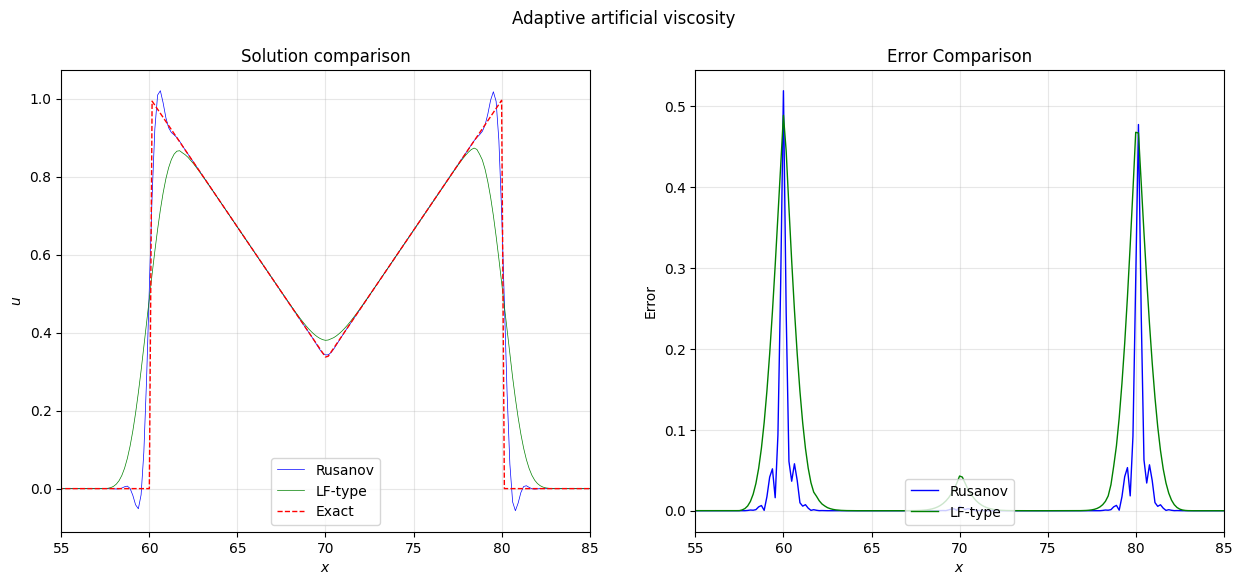
\includegraphics[width=\textwidth]{./src/adaptive-artificial-viscosity.png}
% \caption{Сравнение решений уравнения переноса: схема высокого порядка без коррекции (с осцилляциями) и та же схема с адаптивной искусственной вязкостью.}
\label{fig:adaptive-artificial-viscosity}
\end{figure}

\section{Гибридная схема}
Альтернативный подход к монотонизации состоит в поточечном смешивании решений, полученных по схеме высокого и низкого порядков. Гибридное решение на $(n+1)$-м слое определяется как
\begin{equation}
u^{n+1}_i = w_i\, u^{\text{high}}_i + (1-w_i)\, u^{\text{low}}_i,
\label{eq:hybrid}
\end{equation}
где $u^{\text{high}}_i$ — решение по нашей схеме высокого порядка, $u^{\text{low}}_i$ — решение по монотонной схеме первого порядка (например, схеме против потока), а $w_i \in [0,1]$ — вес, регулирующий вклад высокого порядка. Вес выбирается на основе локального отображения в $[0, 1]$ -- \emph{датчика осцилляций}, который локализует области резких изменений решения. В общем желательно достичь $w_i \approx 1$ на гладких участках и $w_i \approx 0$ вблизи разрывов.

% TODO -- Is it supposed to *theoretically* monotone?
В частности, даже при тривиальном мнгновенном ($w_i \in \{0, 1\}$) переключеннии на схему меньшего порядка в точках изменения знака градиента выходит на практике дает видимое отсутствие эффекта Гиббса.

Для построения весовой функции были реализованы различные датчики осцилляций, включая тривиальное переключение в точках изменения знака градиента~\eqref{eq:oscillation-test}. Все они возвращают значение $S_i \in [0,1]$, где $S_i \approx 1$ указывает на гладкое решение, а $S_i \approx 0$ — на наличие особенности.

\textbf{Датчик кривизны} определён для каждой внутренней ячейки $i = 1,\dots,n-2$ и основан на отношении второй конечной разности к первой:
\begin{equation}
S_i^{\text{cur}} = \frac{|u_{i-1} - 2u_i + u_{i+1}|}{|u_{i-1} - u_i| + |u_i - u_{i+1}| + \varepsilon},
\end{equation}

где $\varepsilon > 0$ — малый параметр, предотвращающий деление на ноль. Датчик принимает значения, близкие к нулю, в точках локального экстремума или излома, и значения порядка единицы на монотонных гладких участках.

\textbf{Датчик вариации} использует расширенный пятиточечный шаблон для ячеек $i = 2,\dots,n-3$:
\begin{equation}
S_i^{\text{var}} = 1 - \frac{|u_{i-1} - 2u_i + u_{i+1}|}{|u_{i+2} - u_{i+1}| + |u_{i+1} - u_i| + |u_i - u_{i-1}| + |u_{i-1} - u_{i-2}| + \varepsilon}.
\end{equation}

Нормировка на сумму вариаций по расширенному шаблону делает датчик менее чувствительным к мелкомасштабным осцилляциям по сравнению с датчиком кривизны, что позволяет лучше отличать слабые разрывы от численного шума. Результат обрезается в диапазон $[0, 1]$.

Пример работы гибридной схемы с очень резким переключением весов показан на рис.~\ref{fig:hybrid}. Видно, что осцилляции полностью исчезают, а разрыв сохраняет высокую крутизну без чрезмерного размазывания.

\begin{figure}[ht]
    \centering
    \input{src/hybrid.tikz}
    % \caption{Сравнение решений: чистая схема высокого порядка, схема первого порядка и гибридная схема. Гибридная комбинация эффективно устраняет осцилляции, сохраняя точность в гладких областях.}
    \label{fig:hybrid}
\end{figure}

Оба метода — адаптивная искусственная вязкость и гибридная схема — позволяют успешно подавить нефизичные осцилляции, однако демонстрируют качественно различное поведение на разрывах. Гибридная схема позволяет добиться более крутого профиля в точке разрыва (см. рис.~\ref{fig:hybrid}), поскольку вблизи особенности решение практически полностью определяется схемой низкого порядка, вносящей меньше дисперсионной ошибки. Дополнительная введеная вязкость же, действуя через добавление диффузионного слагаемого, неизбежно размазывает разрыв на несколько ячеек, даже при адаптивном выборе $\mu$. В гладких областях оба подхода сохраняют высокий порядок.

По вычислительным затратам, минимальный вариант АИВ (предиктор + один корректор) требует трёх вычислений потоков против двух у гибридной схемы; полный трёхпроходный алгоритм АИВ оказывается ещё дороже. С другой стороны, оптимальный метод смешивания схем варьируется от задаче к задаче и вязкость лучше сохраняет устойчивость. 

% Выбор конкретного подхода может определяться требованиями простоты реализации, вычислительной стоимости и конкретной решаемой задачей.

\chapter{Заключение}
\label{sec:conclusion}

В ходе выполнения работы было построено и детально исследовано новое семество сквозных разностных схем, полученных параметрической модификаций схемы Лакса--Фридрихса с привлечением пятиточечного пространственного шаблона. Основные результаты сводятся к следующему.

1. Предложено семейство схем, параметризованных величиной $\sigma$, что позволяет плавно управлять уровнем диссипации и дисперсии метода, выбирая оптимальный баланс под конкретную задачу.

2. Путем тейлоровского разложения и коррекции старшего члена ошибки получена схема, обладающая локальным четвёртым порядком аппроксимации по пространству. Численные эксперименты подтвердили, что интегральная ошибка убывает как $O(\Delta x^3)$.

3. На основе спектрального метода фон~\mbox{Неймана} выполнен исчерпывающий анализ устойчивости. С использованием средств компьютерной алгебры получено замкнутое выражение для множителя перехода $G(\theta,\nu,\sigma)$, аналитически исследована его зависимость от волнового числа и параметров схемы. Определена кривая критического числа Куранта $\nu_{\max}(\sigma)$.

4. Для устранения нефизичных осцилляций на разрывных решениях реализованы два метода монотонизации: адаптивная искусственная вязкость и гибридизация схемы, позволяющая динамически комбинировать решения высокого и низкого порядков. Оба подхода продемонстрировали способность уменьшить ошибку Гиббса, сохраняя достаточно высокую точность на гладких профилях.

5. Полученную сквозную схему легко обобщить на многомерный случай, причем результат также может быть исследован и монотонизирован аналогичными методами.

Проведённое исследование показывает, что предложенная схема сочетает высокую точность, контролируемую устойчивость и возможность монотонизации, что делает её перспективной для решения прикладных задач переноса и гидродинамики. Дальнейшее развитие работы может быть направлено на адаптацию к нелинейным задачам с ударными волнами.

\clearpage

\bibliographystyle{plain}
% \renewcommand\bibname{Reference}

% \chapter*{Список использованных источников}
% \addcontentsline{toc}{chapter}{Список использованных источников}
\begin{thebibliography}{99}
\addcontentsline{toc}{chapter}{Литература}
\bibitem{godunov1954}
Godunov~S.\,K. Different Methods for Shock Waves: Ph.D. Dissertation. --- Moscow State University, 1954.

% \bibitem{godunov1959}
% Годунов~С.\,К. Разностный метод численного расчета разрывных решений уравнений гидродинамики~// Матем. сб. --- 1959. --- Т.~47, \No~3. --- С.~271--306.

\bibitem{rusanov1970}
Rusanov~V.\,V. On difference schemes of third order accuracy for nonlinear hyperbolic systems~// Journal of Computational Physics. --- 1970. --- Vol.~5, Issue~3. --- P.~507--516.

\bibitem{vonneumann1950}
Neumann~J.~von, Richtmyer~R.\,D. A method for the numerical calculation of hydrodynamic shocks~// Journal of Applied Physics. --- 1950. --- Vol.~21, no.~3. --- P.~232--257.

\bibitem{samarsky1971}
Самарский~А.\,А. Теория разностных схем. --- М.: Наука, 1971. --- 553~с.

\bibitem{godunov1977}
Годунов~С.\,К., Рябенький~В.\,С. Разностные схемы (введение в теорию): учебное пособие. --- М.: Главная редакция физико-математической литературы изд-ва \flqq Наука\frqq, 1977.


\bibitem{popov2015}
Попов~И.\,В., Фрязинов~И.\,В. Метод адаптивной искусственной вязкости численного решения уравнений газовой динамики. --- М.: Красанд, 2015. --- 120~с.

\bibitem{galanin1999}
Галанин~М.\,П., Еленина~Т.\,Г. Тестирование разностных схем для линейного уравнения переноса~// Препринты ИПМ им. М.\,В.~Келдыша. --- 1999. --- No~40.
\end{thebibliography}

\end{document}
